\documentclass[ASNA,twocolumn]{USG}

\usepackage{anyfontsize}
\usepackage{xcolor}
\usepackage{colortbl}
\usepackage{bm}
\graphicspath{{./figures/}{./images/}}

\articletype{RESEARCH ARTICLE}
\received{--}
\revised{--}
\accepted{--}
\journal{Advanced Intelligent Systems}
\volume{0}
\copyyear{2026}
\startpage{1}
\articledoi{pending}

\begin{document}

\title{Execution-Confirmed Cooperative Coverage with Baseline-Preserving Repair in Networked Directional Camera Systems}
\author[1]{[ANONYMIZED FOR REVIEW]}
\authormark{ANONYMOUS AUTHOR(S)}
\titlemark{EXECUTION-CONFIRMED COOPERATIVE COVERAGE}
\address[1]{\orgdiv{[DEPARTMENT TO BE COMPLETED], }\orgname{[INSTITUTION TO BE COMPLETED], }\orgaddress{\country{[COUNTRY TO BE COMPLETED]}}}
\corres{[CORRESPONDING AUTHOR AND EMAIL TO BE COMPLETED]}

\keywords{cooperative coverage | active vision | networked sensing robots | task allocation | execution confirmation}

\abstract[ABSTRACT]{Networked directional cameras can enlarge their collective field of view by coordinated pointing, but a planned viewpoint does not establish that a physical observation has occurred. Actuation, settling, video refresh, pose--frame synchronization, and temporary device unavailability alter when each spatial cell is first observed. This article presents ECR-Cover, an execution-confirmed cooperative coverage method that closes this planning--execution gap. It minimizes the area under the uncovered-cell curve over a fixed horizon while constraining complete-coverage time. Initial planning retains a motion-aware greedy solution as an executable baseline and accepts local changes only when they reduce the robust objective without increasing its completion-time bound. During operation, coverage is recorded only after an acknowledged command, stable pose, dwell, fresh image frame, and measured-pose projection; event-triggered repair is likewise compared with continuing the original queues. Four-camera hardware experiments used 240 stratified transitions to calibrate execution-time bounds and 70 frozen-protocol runs for evaluation. Under nominal conditions, ECR-Cover reduced paired UAC relative to both baselines without degrading T100. In repair ablation, it improved nine of ten paired blocks, preserved the preregistered T100 noninferiority margin, and produced measured-pose, fresh-frame evidence of reassigned coverage before recovery in every repair-on run.}

\maketitle

\section{Introduction}\label{sec:introduction}

Coverage is a basic operation in inspection, infrastructure monitoring, environmental sensing, and search without reliable target priors. A coverage system must distribute finite sensing resources over a spatial domain, decide the order in which regions are visited, and determine when a visit can be counted. Classical coverage planning represents the domain by cells, waypoints, or continuous density functions and then optimizes a geometric surrogate such as travel distance, makespan, or accumulated sensing cost \cite{cortes2004coverage,galceran2013survey,tan2021review}. Multi-robot extensions exploit parallel motion and task allocation to reduce completion time. Recent methods further incorporate local-search improvement, online assignment, concurrent planning and execution, and priority-dependent first-visit delay \cite{wang2024apfcpp,wang2025macplanner,mitra2024ondemand,mitra2025concurrent,lee2026priority}. These developments make the planned routes increasingly responsive, but the state variable used by most planners remains an abstract visit: a node is treated as covered when the route reaches it or when the scheduled action is assumed to finish.

The abstraction is less reliable for networked directional cameras. Such a camera covers space by changing its optical axis rather than translating its base. A single pointing direction may cover many cells, and its value depends on field-of-view geometry, camera placement, and overlap with other viewpoints. The time needed to establish an observation is also more than angular displacement divided by a nominal speed. It includes command delivery, device-dependent and direction-dependent gimbal motion, settling, the prescribed dwell, video refresh, and the association of a usable image with the corresponding pose. A controller may acknowledge a velocity command while the camera is still moving. A pose may satisfy its angular tolerance while the available stream still contains a frame acquired before arrival. Conversely, a fresh frame cannot support spatial coverage if its pose association is absent or too old. The physical observation event therefore lies downstream of the planned viewpoint and downstream of the control command.

This distinction matters for both optimization and evaluation. If coverage is updated at the scheduled arrival time, the objective is calculated from events that may not yet have happened. The resulting first-coverage curve can be optimistic even when every waypoint is eventually reached. If a device becomes temporarily unavailable, immediately replacing its queue with a newly optimized queue introduces a second problem: the replacement may be worse than simply allowing healthy devices to continue their current work. A repair mechanism is useful only when its predicted benefit exceeds the cost and uncertainty of switching, and its claimed effect must be visible in subsequent physical observations. These are not isolated implementation details. Together they form a planning--execution mismatch: the planner reasons over a set of feasible viewpoint--cell relations and predicted completion times, whereas the hardware exposes commands, delayed pose samples, image frames, and availability events.

Active camera networks have addressed high-speed tracking, target handoff, predictive scheduling, and zoom control \cite{e2024wisecam,jiang2021pan,zhang2026capture}. Robust active-perception and resilient allocation studies have separately examined motion uncertainty, perception quality, failures, and temporal constraints \cite{xanthidis2024resivis,choudhury2022dynamic,notomista2022resilient}. Yet these lines of work do not by themselves provide a coverage state that is traceable from a planned pointing command to a measured pose and a newly acquired frame, nor do they require every accepted repair to dominate an executable continuation baseline under the same coverage objective. The missing link is an operational contract between planning, physical execution, and observation evidence.

This article formulates that contract for first effective coverage of a fixed three-dimensional region by networked directional cameras. The region is discretized into equal-weight evaluation cells. The primary metric is the fixed-horizon area under the fraction of uncovered cells, termed the uncovered-area criterion (UAC). UAC accounts for the first observation time of every cell rather than only the last completion event. Complete-coverage time, T100, is imposed as a tail constraint instead of being combined with UAC through a problem-dependent weighted sum. Under the limited interpretation of a stationary target whose initial cell is uniformly distributed and whose first valid observation implies detection, UAC equals a truncated expected detection delay. Without those assumptions it is, more precisely, a truncated first-observation latency and is reported as such throughout the article.

The resulting method, ECR-Cover, links three components. First, initial planning retains a complete motion-aware greedy (MAG) route as a fallback and uses calibrated end-to-end execution-time upper bounds to evaluate deterministic local modifications. A candidate can replace the incumbent only if it preserves complete feasible coverage, strictly reduces robust UAC, and respects the MAG T100 bound. Second, execution uses a state machine in which an acknowledged command, a continuously stable measured pose, a dwell interval, a usable fresh frame, and bounded pose--frame time separation are all required before coverage is recorded. The recorded set is generated by projecting the measured pose associated with that frame; the planned pose never writes coverage directly. Third, temporary unavailability triggers residual-task repair. The already confirmed set is frozen, active tasks on healthy devices are retained, and the candidate repair is compared with the executable policy of continuing the original queues. Repair is committed only when it improves predicted residual UAC beyond a switching threshold, does not increase predicted residual T100, and contains a predicted reassigned observation before the unavailable device can recover.

The contribution is consequently a closed-loop coverage method rather than a new general-purpose optimization theorem. Its formal results are structural properties of the frozen planning model and the implemented evidence rules: (i) the initial planner preserves the MAG baseline in robust UAC and T100; (ii) every logged coverage update has a matching command--pose--frame evidence chain; (iii) coverage completes under explicit reachability, recovery, and eventual-confirmation conditions; and (iv) an accepted repair preserves its original-queue baseline in the predicted residual problem. Hardware results then test whether these model-level properties have useful observable consequences. Four ZR10 pan--tilt cameras supplied 240 stratified transitions for execution-time modeling and 70 runs under frozen nominal, interruption, and repair-ablation protocols. The experiments evaluate first-coverage latency, completion tails, physical evidence consistency, and computation time without using a target detector or target ground truth.


\section{Related Work}\label{sec:related}

\subsection{Cooperative and Multi-Robot Coverage}

Coverage planning spans continuous coverage control, cellular decompositions, graph traversal, sampling-based planning, and data-driven allocation. Continuous formulations distribute mobile sensors according to spatial density functions and provide a foundation for geometric coverage control \cite{cortes2004coverage}. Sensor-based methods instead build decompositions incrementally from local observations \cite{acar2002sensor}. Surveys by Galceran and Carreras and by Tan et al. organize the large body of offline path-planning and heuristic approaches around environment representation, completeness, and path cost \cite{galceran2013survey,tan2021review}. Although these formulations differ in geometry, the coverage event is normally attached to a robot's spatial visit or sensing footprint at a planned configuration.

For multiple robots, workload division and route interaction become central. Artificial-potential-field and integrated assignment--planning approaches construct online routes while discouraging overlap or balancing the remaining region \cite{wang2024apfcpp,wang2025macplanner}. Local-search MCPP starts from a complete solution and improves it with neighborhoods that exchange or reshape route segments \cite{tang2024local}; this baseline-plus-improvement structure is important to the present planner, although ECR-Cover uses different objectives and acceptance tests. Online on-demand MCPP assigns work when execution makes it necessary, while concurrent MCPP reduces idle time by allowing planning and motion to overlap \cite{mitra2024ondemand,mitra2025concurrent}. Priority-aware coverage shifts attention from makespan alone toward when important cells are first reached \cite{lee2026priority}. Field-of-view-aware patrol planning and distribution-matching sensor deployment further show that a sensing footprint can be more informative than a point-robot path \cite{zuo2026fom,ghimire2024stein}. Persistent coverage for random-target search and inspection of complex structures illustrate related applications in which repeated visits or three-dimensional sensing geometry matter \cite{li2025persistent,jing2020multiuav}.

ECR-Cover draws on these ideas but addresses a different boundary. Its cameras are fixed in position and create coverage through pointing, so a viewpoint is a set-cover action rather than a translational cell visit. More importantly, planned feasibility and executed observation are represented by separate sets. The method does not alter the basic combinatorial difficulty of multi-agent coverage; it supplies a retained feasible baseline, a first-observation objective, and an observation-evidence interface that can be audited after execution.

\subsection{Active and Networked Camera Systems}

Pan--tilt camera research has produced systems with rapid visual feedback, target prediction, and coordinated viewpoint control. WiseCam develops systematic intelligence for pan--tilt tracking in networked settings, while high-frame-rate pan--tilt platforms couple object detection with fast actuation \cite{e2024wisecam,jiang2021pan}. Predictive scheduling and zoom control extend this direction to multi-target capture over large scenes \cite{zhang2026capture}. These systems demonstrate that camera motion, image timing, and network organization cannot be separated in a physical implementation. Their central objective, however, is usually maintaining target visibility or acquiring detailed target imagery, not certifying the first valid observation time of every spatial cell.

Multi-robot reconstruction and task-relevant exploration provide a second connection. Centralized and distributed reconstruction systems coordinate viewpoints to acquire complementary surface information \cite{hardouin2023reconstruction}; semantic Gaussian-splatting methods use scene content to guide reconstruction or exploration \cite{zeng2025multirobot,nagami2026vista}. Robust active-perception planners such as ResiVis explicitly account for uncertainty in motion and perception quality \cite{xanthidis2024resivis}. These approaches make observation value part of the planning problem. ECR-Cover is deliberately more modest in perception semantics: it does not infer target identity, reconstruction quality, or detection probability. Its observation predicate is instead operational. A cell is counted only when a usable frame acquired after stable arrival can be associated with a measured pose whose projected field of view contains that cell in the frozen camera model.

This operational definition helps separate two questions that are often conflated. Geometric feasibility asks whether a candidate pointing direction can cover a cell under the planning map. Physical confirmation asks whether the real device produced qualifying evidence for that cell during the run. A calibrated or conservative planning map may improve the former, but it cannot substitute for the latter. The distinction is particularly important with RTSP streams, for which command acknowledgment and image freshness belong to different network paths.

\subsection{Execution Uncertainty and Resilient Allocation}

Uncertain execution has been treated through stochastic scheduling, robust optimization, online replanning, and resilient assignment. Dynamic multi-robot task allocation incorporates uncertainty and temporal constraints when deciding which robot should perform a task \cite{choudhury2022dynamic}. Resilient and energy-aware allocation maintains team function under heterogeneous capabilities and robot failures \cite{notomista2022resilient}. Large-neighborhood search provides a general mechanism for starting with a feasible route and repeatedly destroying and repairing parts of it while retaining the best verified incumbent \cite{ropke2006alns}. ECR-Cover uses a small deterministic neighborhood rather than adaptive large-neighborhood search, but shares the crucial anytime principle that an interrupted search must return a validated incumbent.

The execution-time model also relates to calibrated prediction. Conformal prediction gives finite-sample marginal coverage statements under exchangeability, and Mondrian variants condition calibration on predefined groups \cite{angelopoulos2023conformal,bostrom2021mondrian}. Here, transfers are grouped by angular range so that residuals from large motions do not dominate short transfers. This construction supplies one-sided empirical margins for end-to-end time, but the formal coverage propositions do not assume that future data are automatically exchangeable. They explicitly condition on realized task times not exceeding the calibrated upper bounds. This wording keeps the role of calibration distinct from the deterministic baseline-preserving logic.

Two gaps remain when the above areas are considered together. First, a route planner can be robust with respect to its timing model and still mark a cell from a stale frame. Second, a resilient allocator can generate a plausible replacement assignment without showing that the replacement improves the coverage trajectory relative to leaving healthy queues unchanged. ECR-Cover addresses these gaps by treating the original complete route and original residual queues as executable baselines, and by making measured-pose, fresh-frame confirmation the only operation that changes the realized coverage state.


\section{Problem Formulation}\label{sec:problem}

\subsection{Spatial Cells, Candidate Viewpoints, and Feasible Coverage}

Let $\mathcal R=\{1,\ldots,N\}$ be the set of directional camera devices. The evaluation region is represented by $M$ equal-weight cell centers $\mathcal C=\{\mathbf x_m\}_{m=1}^{M}$. Device $i$ has a finite candidate-viewpoint set $\mathcal Q_i$. A viewpoint $q=(\theta_{iq},\phi_{iq})$ specifies azimuth and elevation in the device's control coordinate system. Given the device pose, mounting rotation, camera intrinsics, and fixed zoom, the pinhole model maps each candidate to a nominal cell set $\mathcal B_{iq}$. These quantities define a common frozen geometry for all compared planning methods.

The planner operates on an admissible map $\mathcal B^{\mathrm a}_{iq}\subseteq\mathcal B_{iq}$. This separation is useful because the propositions require only that all methods use the same frozen map; they do not require a particular construction. In the hardware implementation, the map was generated from the completion tolerance of the pose controller. Let
$\mathcal D_i=[-e_i^\theta,e_i^\theta]\times[-e_i^\phi,e_i^\phi]$, where $e_i^\theta$ and $e_i^\phi$ are azimuth and elevation half-widths and $\operatorname{corners}(\mathcal D_i)$ denotes the four corners of the error box. The implemented planning core is

\begin{equation}\label{eq:safety-core}
\mathcal B^{\mathrm s}_{iq}=
\bigcap_{(\delta_\theta,\delta_\phi)\in\operatorname{corners}(\mathcal D_i)}
\mathcal B_i(\theta_{iq}+\delta_\theta,\phi_{iq}+\delta_\phi),
\qquad \mathcal B^{\mathrm a}_{iq}=\mathcal B^{\mathrm s}_{iq}.
\end{equation}

Equation~\eqref{eq:safety-core} is a practical four-corner intersection used by the frozen implementation. It reduces dependence on cells lying at the nominal field-of-view boundary. It is not a physical confidence region for the camera footprint: station coordinates, mounting extrinsics, and per-camera intrinsic errors were not jointly calibrated against external ground truth. It is also not the principal algorithmic contribution. Replacing it with another frozen feasible map would leave the baseline-preserving proofs unchanged, provided that all compared plans were evaluated on that same map.

A route for device $i$ is an ordered sequence $\pi_i=(q_{i1},\ldots,q_{iK_i})$, and a team plan is $\Pi=\{\pi_i\}_{i=1}^{N}$. The planning task is feasible only if the union of admissible candidate sets covers all cells. Feasibility is checked before route construction. During execution, $\mathcal B^{\mathrm a}_{iq}$ can justify assigning a viewpoint but cannot itself create a realized coverage record; that record is defined from measured-pose evidence in Section~\ref{sec:method}.

\subsection{End-to-End Execution-Time Upper Bound}

The duration of a viewpoint task begins with the first relevant control command and ends only after continuous pose stability, the prescribed dwell, and acquisition of a new frame at the arrived pose. This definition includes more than mechanical movement and is aligned with the event that can establish coverage. For a transfer from $q$ to $q'$ on device $i$, the point prediction is the nonnegative monotone model

\begin{equation}\label{eq:time-point}
\begin{split}
\hat\tau_i(q,q')={}&\beta_{i0}+\beta_{i\theta+}[\Delta\theta]_+
+\beta_{i\theta-}[-\Delta\theta]_+\\
&+\beta_{i\phi+}[\Delta\phi]_+
+\beta_{i\phi-}[-\Delta\phi]_+
+\beta_{ic}\,\mathbb I_{2\mathrm a},
\end{split}
\end{equation}

where $[x]_+=\max(x,0)$, $\Delta\theta$ and $\Delta\phi$ are wrapped azimuth and elevation changes, and $\mathbb I_{2\mathrm a}$ indicates simultaneous two-axis motion. All coefficients are constrained to be nonnegative and are fitted by Huber-weighted nonnegative least squares. Separate positive and negative coefficients allow direction-dependent device behavior without permitting a physically implausible decrease in predicted time as a single-axis displacement grows.

Transfers are divided by $d=\max(|\Delta\theta|,|\Delta\phi|)$ into small ($d\leq3^\circ$), medium ($3^\circ<d\leq12^\circ$), and large ($d>12^\circ$) angular ranges. One-sided residual quantiles $r_g$ are computed on calibration runs that are disjoint from fitting runs. The planning upper bound is

\begin{equation}\label{eq:time-upper}
\bar\tau_i(q,q')=\max\{\tau_{\min},\hat\tau_i(q,q')+r_{g(q,q')}\}.
\end{equation}

Grouping prevents the residual spread of large transfers from setting every short-transfer margin. If future transfers are exchangeable with the calibration examples within their assigned group, Equation~\eqref{eq:time-upper} admits a finite-sample marginal-coverage interpretation. The deterministic results below use a simpler explicit condition: the realized end-to-end duration of each executed task does not exceed its corresponding $\bar\tau_i$. Thus a departure from the calibration regime affects the tightness and empirical validity of the time bound, but not the internal logic of retaining an evaluated baseline.

\subsection{First Effective Coverage Objective}

Let $a_{ik}$ be the predicted confirmation time of the $k$th viewpoint on device $i$, obtained by recursively summing Equation~\eqref{eq:time-upper} from the initial pose through the route. The planning-time first-coverage upper bound for cell $m$ is

\begin{equation}\label{eq:first-time}
\bar T_m(\Pi)=
\min_{i,k:\,m\in\mathcal B^{\mathrm a}_{iq_{ik}}} a_{ik}.
\end{equation}

For a fixed evaluation horizon $H$, define the robust uncovered-area criterion

\begin{equation}\label{eq:uac}
\overline{\mathrm{UAC}}_H(\Pi)
=\frac{1}{M}\sum_{m=1}^{M}\min\{\bar T_m(\Pi),H\}
=\int_0^H[1-\bar C(t)]\,\mathrm dt,
\end{equation}

where $\bar C(t)=M^{-1}\sum_m\mathbb I[\bar T_m\leq t]$ is the predicted covered fraction. The realized metric $\mathrm{UAC}_H$ replaces $\bar T_m$ with the execution-confirmed time $T_m$. The truncation makes unfinished cells contribute the full horizon rather than disappear as missing observations. It also prevents early termination from improving the metric artificially.

UAC has a probabilistic interpretation only under stated conditions. If a target is stationary during the task, its initial cell is uniformly distributed over the equal-weight cells, and the first effective observation of that cell guarantees detection, then $\mathrm{UAC}_H=\mathbb E[\min(T,H)]$. For an unknown moving target or an unknown detector, the equality does not hold. The metric then describes the latency distribution of spatial observation opportunities, not detection probability.

Two tail summaries accompany UAC. $T_{95}$ is the 95th percentile of $\{T_m\}$ and $T_{100}=\max_m T_m$ is complete-coverage time. ECR-Cover solves

\begin{equation}\label{eq:optimization}
\begin{split}
\min_{\Pi}\quad &\overline{\mathrm{UAC}}_H(\Pi),\\
\mathrm{s.t.}\quad &\bigcup_{i,q\in\pi_i}\mathcal B^{\mathrm a}_{iq}=\mathcal C,\\
&\bar T_{100}(\Pi)\leq \bar T_{100}(\Pi_{\mathrm{MAG}}),
\end{split}
\end{equation}

where $\Pi_{\mathrm{MAG}}$ is a complete motion-aware greedy plan built from the same admissible map and initial poses. UAC is the sole primary objective. $T_{95}$, total angular motion, and the coefficient of variation of device load are deterministic tie-break quantities; they cannot override the UAC improvement or T100 constraint.

\begin{figure*}[t]
\centering
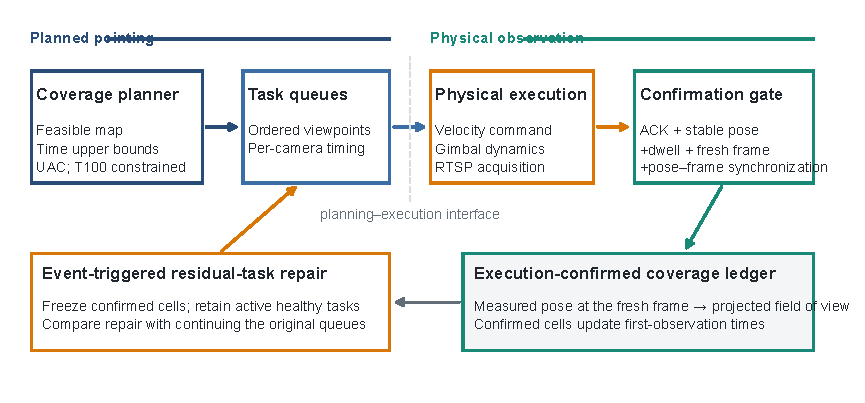
\includegraphics[width=\textwidth]{figure1_system_loop.pdf}
\caption{The ECR-Cover planning--execution--observation loop. Planning produces timed viewpoint queues from a frozen feasible map and end-to-end time bounds. Physical coverage is updated only after command acknowledgment, stable pose, dwell, a fresh usable frame, and pose--frame synchronization. Availability events invoke residual-task repair, but the original queues remain the executable comparison baseline.}\label{fig:system-loop}
\end{figure*}


\section{ECR-Cover}\label{sec:method}

\subsection{System-Level Planning--Execution--Observation Loop}

ECR-Cover maintains two related but noninterchangeable states (Figure~\ref{fig:system-loop}). The planning state contains candidate viewpoints, admissible cell sets, predicted end-to-end durations, and ordered queues. The physical state contains device availability, command results, pose samples, frame records, and the cells that have been confirmed. A planned cell can influence route selection; only a confirmed cell can influence the realized coverage curve. This separation prevents the planner from manufacturing evidence by advancing its own clock.

The same distinction governs repair. When availability changes, the residual problem is built from the confirmed set rather than from the set that the original schedule expected to have covered. Healthy devices continue their current actions while a bounded planner evaluates alternatives. The result is an anytime loop: an executable plan exists before search begins, and a time limit stops search without promoting an unchecked candidate. The initial and event-driven phases use different baselines because their operational alternatives differ. Before execution, MAG is the complete reference route. During execution, the relevant alternative is continuing the queues that are already in progress.

\subsection{Baseline-Preserving Initial Planning}

The initial MAG route is constructed deterministically. At each step, a candidate viewpoint is appended according to the ratio between marginal admissible coverage and nominal maneuver cost until all cells are assigned. MAG supplies both an executable fallback and the fixed T100 ceiling in Equation~\eqref{eq:optimization}. A second complete seed uses the calibrated bounds in Equation~\eqref{eq:time-upper}. Starting from these seeds, ECR-Cover searches three neighborhoods in a fixed order: removal of a redundant viewpoint, relocation within one device route, and viewpoint replacement or migration across devices. Whenever an improvement is accepted, search restarts from the first neighborhood. This ordering makes the run reproducible and prioritizes deletion of work that no longer contributes to first coverage.

For current plan $\Pi$, candidate $\Pi'$, and numerical tolerance $\varepsilon$, acceptance requires

\begin{equation}\label{eq:initial-accept}
\begin{aligned}
&\bigcup_{i,q\in\pi_i'}\mathcal B^{\mathrm a}_{iq}=\mathcal C,\\
&\overline{\mathrm{UAC}}_H(\Pi')
<\overline{\mathrm{UAC}}_H(\Pi)-\varepsilon,\\
&\bar T_{100}(\Pi')
\leq\bar T_{100}(\Pi_{\mathrm{MAG}})+\varepsilon.
\end{aligned}
\end{equation}

The implementation also applies the same nonincrease condition to T100 under the nominal, uncontracted field-of-view map. This additional check prevents overlapping admissible sets from making a viewpoint appear redundant when it remains useful to the execution tail. Search is bounded by a fixed number of evaluations and a 200~ms wall-clock budget. When either limit is reached, the last verified incumbent is returned.

\begin{proposition}[Baseline preservation in initial planning]\label{prop:initial}
If $\Pi_{\mathrm{MAG}}$ completely covers $\mathcal C$, ECR-Cover returns a complete plan $\Pi^*$ at any planning-budget termination, and
\begin{equation}\label{eq:initial-property}
\overline{\mathrm{UAC}}_H(\Pi^*)
\leq\overline{\mathrm{UAC}}_H(\Pi_{\mathrm{MAG}}),\qquad
\bar T_{100}(\Pi^*)
\leq\bar T_{100}(\Pi_{\mathrm{MAG}}).
\end{equation}
\end{proposition}

\begin{proof}
The initial incumbent is the complete plan $\Pi_{\mathrm{MAG}}$. Equation~\eqref{eq:initial-accept} ensures that every accepted incumbent remains complete, strictly reduces robust UAC, and stays below the fixed MAG T100 ceiling. Rejected candidates do not modify the incumbent. Terminating on the evaluation or wall-clock budget interrupts search but does not replace the last verified plan. The two inequalities and completeness therefore hold by induction over the finite accepted sequence.
\end{proof}

The proposition is relative to the same admissible coverage map and the same time bounds. It does not say that the returned plan is globally optimal, nor that its realized hardware UAC must be lower than MAG in every run. Those questions depend on model fit and physical execution and are examined experimentally.

\subsection{Execution-Confirmed Coverage}

Each device executes a viewpoint through five stages: MOVE, SETTLE, DWELL, FRAME-CONFIRM, and COMPLETE. MOVE closes the velocity command loop around live pose measurements; an ACK indicates command-path success but not arrival. SETTLE begins only after pose error and angular velocity remain below their thresholds for a continuous stability window. The camera then completes the required dwell. FRAME-CONFIRM requests frames created after arrival and admits them only if they pass availability, resolution, brightness, contrast, and sharpness checks. The host-side acquisition time of the final frame must lie within the synchronization tolerance of the associated pose sample.

Let $e_{ik}=1$ indicate that task $k$ of device $i$ has passed this sequence, $t^c_{ik}$ its completion time, and $\widehat{\mathcal B}_{ik}$ the cell set obtained by projecting the measured pose associated with the confirming frame. Realized coverage is

\begin{equation}\label{eq:confirmed-state}
y_m(t)=\mathbb I\!\left[\exists(i,k): e_{ik}=1,\;
m\in\widehat{\mathcal B}_{ik},\;t^c_{ik}\leq t\right].
\end{equation}

The realized first-coverage time is the earliest $t$ for which $y_m(t)=1$. If no valid evidence is obtained before $H$, the cell remains unconfirmed for the UAC calculation even if the route expected it to be covered. The ledger stores the task identifier, command outcome, stability samples, frame identifier and timestamp, matched pose, projected cell set, and completion event. These fields permit the coverage curve to be reconstructed without invoking the planner's nominal arrival time.

\begin{proposition}[Model-internal consistency of coverage records]\label{prop:evidence}
If Equation~\eqref{eq:confirmed-state} marks cell $m$ as covered at time $t$, the log contains, for the same task, a successful command result, a continuously stable measured pose, a usable frame acquired after arrival, and a pose sample within the synchronization tolerance of that frame; under the frozen projection model, $m$ belongs to the field of view projected from that pose.
\end{proposition}

\begin{proof}
The ledger is updated only on entry to COMPLETE. The state machine cannot enter COMPLETE until the command, stability, dwell, frame-freshness, frame-quality, and synchronization gates have all passed. The update writes only members of $\widehat{\mathcal B}_{ik}$, which is calculated from the measured pose associated with the final frame. Failure of any preceding gate prevents the write.
\end{proof}

This is a statement about the consistency of software events with a frozen camera model. It is not an external calibration theorem. In particular, it does not establish absolute world-coordinate footprint accuracy when station, mounting, or intrinsic parameters contain unmodeled errors.

\begin{proposition}[Conditional completeness]\label{prop:complete}
Suppose the union of the admissible candidate sets equals $\mathcal C$, unavailable devices recover in finite time, and every dispatched reachable task eventually completes execution confirmation. ECR-Cover confirms every cell after finitely many effective task completions.
\end{proposition}

\begin{proof}
Candidate viewpoints and cells are finite. Each effective completion either confirms at least one previously unconfirmed cell or exhausts a finite task that has become redundant because another confirmed viewpoint already covers its contribution. Repair never removes confirmed coverage. The residual unconfirmed set is therefore monotone nonincreasing and, under eventual completion of reachable dispatched tasks and finite recovery, reaches the empty set after finitely many effective completions.
\end{proof}

\begin{figure*}[t]
\centering
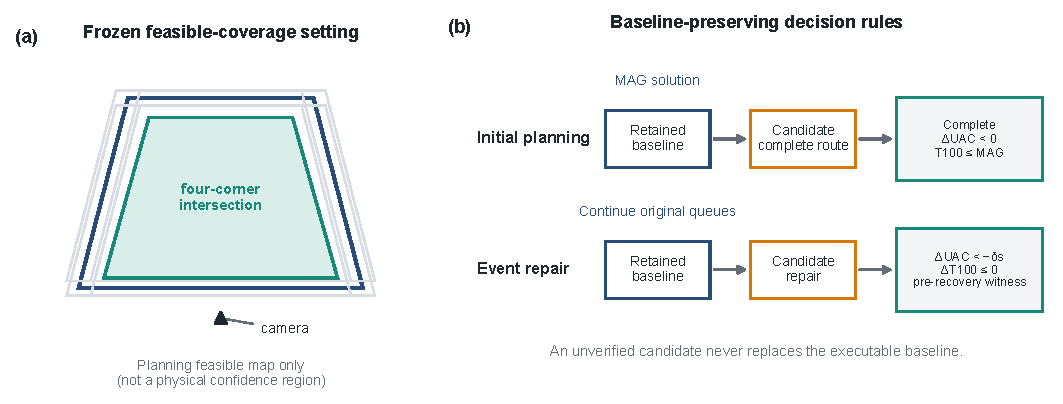
\includegraphics[width=\textwidth]{figure2_baseline_rules.pdf}
\caption{Frozen feasible-coverage setting and baseline-preserving decisions. (a) The implementation uses a four-corner field-of-view intersection as the common planning map; it is not interpreted as a physical confidence region and does not create realized coverage. (b) Initial search retains MAG, whereas event repair retains continuation of the original queues. A candidate replaces its baseline only after the corresponding UAC and T100 checks pass.}\label{fig:baseline-rules}
\end{figure*}

\subsection{Event-Triggered Residual-Task Repair}

A device-unavailable event freezes the confirmed set and marks the device's uncompleted tasks as temporarily unavailable. Tasks currently running on healthy devices and their remaining queues are retained. Let $\mathcal U$ be the set of unconfirmed cells. Among tasks in the unavailable device's original queue, only cells not already covered by the remaining healthy queues form the transferable set $\mathcal X\subseteq\mathcal U$. This rule avoids perturbing healthy work for cells that are already scheduled elsewhere.

The residual timing origin for each healthy device is its predicted pose and conservative remaining duration after the currently active task. Continuing the retained queues defines the executable baseline $\Pi^0$. The repair search inserts viewpoints that can cover $\mathcal X$ into healthy queues, with no more than three accepted insertions and a 40~ms wall-clock budget. Let $\Pi^+$ be a candidate and $\delta_s$ the switching threshold. It is committed only if

\begin{equation}\label{eq:repair-accept}
\overline{\mathrm{UAC}}_H(\Pi^+)
<\overline{\mathrm{UAC}}_H(\Pi^0)-\delta_s,
\qquad
\bar T_{100}(\Pi^+)\leq\bar T_{100}(\Pi^0).
\end{equation}

In addition, at least one transferred cell must have a predicted confirmation time earlier than the unavailable device's earliest recovery time minus margin $\delta_w$. This pre-recovery witness links a queue change to an observable opportunity that could not arise merely by waiting for the original device. The recovery event uses the same baseline comparison before tasks are returned, which avoids oscillation caused by a device briefly reappearing. Planning runs concurrently with the healthy devices' current actions; an event on one device therefore does not impose a team-wide planning pause.

\begin{proposition}[Baseline preservation in event repair]\label{prop:repair}
Every committed repair reduces predicted residual UAC relative to $\Pi^0$ by at least $\delta_s$, does not increase predicted residual T100, and contains a predicted reassigned-coverage witness before recovery.
\end{proposition}

\begin{proof}
The original-queue continuation $\Pi^0$ remains executable while the bounded search evaluates candidates. A candidate replaces it only after Equation~\eqref{eq:repair-accept} and the pre-recovery witness check pass. The stated properties are therefore invariants of the commit operation. They concern the calibrated residual model; whether the witness becomes a confirmed hardware observation is tested from the execution ledger.
\end{proof}

\subsection{Scope of the Formal Properties}

The four propositions occupy different evidential levels. Proposition~\ref{prop:initial} is a planning invariant: it compares two plans under a shared admissible map and time model. Proposition~\ref{prop:evidence} is a log-to-model consistency statement: it connects a coverage write to the measurements required by the implementation. Proposition~\ref{prop:complete} is conditional and makes the reachability and eventual-completion assumptions explicit. Proposition~\ref{prop:repair} is again a planning invariant, now for the residual problem. None alone proves physical superiority over a baseline. Physical superiority requires frozen, paired hardware observations, while physical geometric accuracy would require external calibration evidence not available in the present platform. Keeping these levels separate is essential to the interpretation of the experiments.


\section{Experimental System and Methods}\label{sec:experiments}

\subsection{Four-Camera Platform and Frozen Geometry}

The platform comprises four ZR10 pan--tilt cameras connected to one control computer. The controller runs at 10~Hz in the \texttt{velocity\_p} mode and receives four RTSP streams. In the frozen local model, camera positions are $(-5,-5,1.5)$, $(-5,5,1.5)$, $(5,5,1.5)$, and $(5,-5,1.5)$~m. The evaluation volume is $[112,128]\times[-8,8]\times[52,68]$~m and is discretized into an $8\times12\times4$ grid, giving 384 equal-weight cells. All cameras use fixed 10$\times$ zoom and a configured resolution of $1920\times1080$. Candidate commands obey azimuth limits of $[-35^\circ,35^\circ]$ and elevation limits of $[-20^\circ,20^\circ]$.

These coordinates constitute one internally consistent local geometry for planning and log reconstruction. They are not used to claim absolute world-coordinate pointing accuracy. The admissible map in Equation~\eqref{eq:safety-core} is shared by ECR-Cover, MAG, and the calibrated static baseline, so between-method effects cannot be attributed to different field-of-view contractions.

\subsection{Execution-Confirmation Thresholds}

A viewpoint reaches the stable-pose gate when measured azimuth and elevation are within $1^\circ$ of the command and angular speed is below $0.8^\circ$~s$^{-1}$ continuously for 0.35~s. The device then dwells for 0.8~s. Confirmation requires at least three new frames, a frame--pose time difference no greater than 0.2~s, and a fresh-frame wait no longer than 2~s. Frame records also pass availability, resolution, brightness, contrast, and sharpness checks before they can support coverage.

The $1^\circ$ planning half-width was tied to the implemented completion gate and observed pose errors. On 48 independent calibration transfers, the median, 95th percentile, and maximum azimuth arrival errors were $0.667^\circ$, $0.941^\circ$, and $1.000^\circ$; the corresponding elevation values were $0.469^\circ$, $0.870^\circ$, and $0.893^\circ$. On the 48 independent test transfers, the maximum azimuth and elevation errors were $0.891^\circ$ and $0.889^\circ$. Accordingly, $e_i^\theta=e_i^\phi=1^\circ$ was used for all four devices. The value is a completion tolerance in the control and telemetry coordinates, not a confidence bound for all camera-model errors.

The geometric effect of this choice was quantified offline on the frozen model without changing any hardware result. Table~\ref{tab:core-sensitivity} varies the half-width and recomputes candidate coverage and the initial ECR-Cover plan. At $1^\circ$, the median candidate covers 56 cells rather than 138 under the nominal map, and the planned route contains 16 rather than 5 tasks. This sensitivity check explains that the chosen map is consequential, but it is not a hardware comparison among tolerance settings.

\subsection{Execution-Time Calibration}

Each camera performed 60 stratified transfers, for 240 total. The transfer set covered the small, medium, and large angular groups and both signs of azimuth and elevation motion. For each device, 36 complete-run samples were used for model fitting, 12 disjoint complete-run samples for residual calibration, and 12 further complete-run samples only for testing. A run never contributed observations to more than one split. This run-level separation avoids allowing closely related records from the same execution to enter both fitting and calibration.

Table~\ref{tab:time-model} reports the independent test results. The upper-bound coverage column is the fraction of test transfers whose complete command-to-fresh-frame duration did not exceed Equation~\eqref{eq:time-upper}. The experiment targeted a one-sided 90\% level. Prediction error remains material because the response includes settling and frame acquisition rather than only gimbal travel. The method therefore uses the calibrated bound for planning instead of treating a nominal angular speed as an execution clock.

\begin{table*}[t]
\caption{Independent test results for the end-to-end execution-time model.}\label{tab:time-model}
\centering
\begin{tabular}{cccccc}
\toprule
Device & Test transfers & MAE (s) & RMSE (s) & Upper-bound coverage (\%) & Mean upper margin (s)\\
\midrule
ZR10-1 & 12 & 3.262 & 3.719 & 100.0 & 5.917\\
ZR10-2 & 12 & 3.977 & 4.655 & 91.7  & 5.917\\
ZR10-3 & 12 & 4.458 & 5.367 & 83.3  & 6.098\\
ZR10-4 & 12 & 5.229 & 7.469 & 83.3  & 6.823\\
\midrule
Aggregate/mean & 48 & 4.231 & 5.302 & 89.6 & 6.188\\
\bottomrule
\end{tabular}
\end{table*}

\begin{table*}[t]
\caption{Offline sensitivity of the planning feasible map in the frozen geometry. The analysis changes only the planning-map half-width; it does not add hardware trials.}\label{tab:core-sensitivity}
\centering
\begin{tabular}{cccccc}
\toprule
Half-width (deg) & Median cells/view & Median retained (\%) & Planned tasks & Planned UAC (s) & Planned T100 (s)\\
\midrule
0.0 & 138 & 100.0 & 5  & 4.816  & 17.886\\
0.5 & 94  & 68.7  & 8  & 6.394  & 21.486\\
1.0 & 56  & 40.3  & 16 & 9.970  & 40.348\\
1.5 & 24  & 16.2  & 33 & 17.204 & 85.519\\
\bottomrule
\end{tabular}
\end{table*}

\subsection{Experimental Protocol and Research Questions}

The evaluation horizon was fixed at $H=60$~s and each run recorded 85~s of system activity. Before a run, the controller checked all four poses, zoom values, video streams, and configuration hashes. After a run, all devices returned to their home poses. A complete physical run, not a control cycle, frame, event, or cell, is the statistical unit.

Nominal evaluation used ten randomized blocks. Each block contained ECR-Cover, MAG, and a calibrated static method that used Equation~\eqref{eq:time-upper} to construct its initial route but never modified the queue during execution. These 30 runs addressed whether ECR-Cover improves run-level first-coverage latency without worsening the completion tail.

Interruption trials logically paused an active device for 25~s when confirmed coverage first reached 50\%. The paused device was selected by a frozen rule: among active devices, choose the one owning the greatest number of uniquely covered remaining cells. One ten-block experiment compared ECR-Cover with the calibrated static method under this interruption. Because that comparison changes both initial route and repair behavior, it is reported as a system-level comparison rather than evidence isolating repair. A second ten-block experiment held the initial ECR-Cover route, pause rule, and evidence logic fixed and paired repair enabled with repair disabled. This repair-on/off ablation is the primary test of the repair mechanism. Across nominal, interrupted-baseline, and repair-ablation protocols, 70 hardware runs were completed.

The experiments were organized around four questions. RQ1 asks how well the grouped end-to-end bounds describe independent transfers. RQ2 asks whether the baseline-preserving initial planner reduces nominal UAC while maintaining T100. RQ3 asks whether event repair, isolated by the switch ablation, changes UAC and remains noninferior in T100. RQ4 asks whether the events supporting coverage and reassignment are traceable to measured poses and fresh frames, and whether planning respects its wall-clock budgets.

\subsection{Statistical Analysis}

All reported summaries are calculated at the run level. For each method, continuous outcomes are presented as the median and interquartile range (IQR), with the ten original observations retained in the figures. Paired effects use within-block differences or ratios. The reported 95\% confidence intervals were produced by 100000 block-level bootstrap resamples under the frozen analysis. Directional primary hypotheses use the preregistered one-sided exact sign test. For nominal coverage, the principal comparison is ECR-Cover minus MAG UAC; the calibrated-static comparison characterizes the additional gain over a time-aware fixed route. For repair ablation, the principal effect is repair-on minus repair-off UAC. T100 is evaluated against the frozen 5\% noninferiority margin using the paired repair-on/off ratio. T95, total angular motion, load coefficient of variation, frame waiting, and planning time are secondary descriptive outcomes. Runs that failed to complete within $H$ would contribute censored first-coverage times at $H$ through Equation~\eqref{eq:uac}; no such run was discarded or replaced in the reported 70-run set. The plotting code displays the frozen intervals and does not recalculate them with an alternative statistical procedure.


\section{Results}\label{sec:results}

\subsection{Execution-Time Model}

Across the 48 independent test transfers, 43 end-to-end durations fell below their grouped upper bounds, giving an aggregate empirical coverage of 89.6\%, close to the intended 90\% one-sided level (Table~\ref{tab:time-model}). Per-device coverage ranged from 83.3\% to 100.0\%. Mean upper margins were 5.917--6.823~s, while MAE ranged from 3.262 to 5.229~s and RMSE from 3.719 to 7.469~s. These errors are large relative to a purely mechanical short transfer because the response variable includes command handling, closed-loop arrival, stability, dwell, and the first qualifying post-arrival frame. The result supports using device- and direction-dependent end-to-end bounds in the planner; it does not establish an unconditional timing guarantee under network conditions outside the calibration runs.

The offline field-of-view sensitivity in Table~\ref{tab:core-sensitivity} shows a separate effect. A $1^\circ$ half-width retained a median 40.3\% of nominal cells per candidate and increased the planned task count from 5 to 16 relative to the uncontracted map. Its planned UAC and T100 were therefore higher than those at $0^\circ$ or $0.5^\circ$. The analysis clarifies the planning cost of the frozen feasible map. Because no hardware run was repeated under the alternative half-widths, the table cannot establish which half-width would yield the best physical performance.

\subsection{Nominal First-Coverage Performance}

All 70 hardware runs confirmed all 384 cells. Table~\ref{tab:nominal} summarizes the 30 nominal runs. Median UAC was 2.380~s for ECR-Cover, 7.480~s for MAG, and 3.070~s for the calibrated static route. The paired ECR-Cover-minus-MAG UAC median was $-4.941$~s with a 95\% bootstrap CI of $[-6.707,-3.910]$~s. All ten blocks favored ECR-Cover, giving a one-sided exact sign-test value of $p=0.0009766$. Relative to calibrated static planning, the paired median difference was $-0.265$~s with a 95\% CI of $[-1.046,-0.110]$~s. Figure~\ref{fig:nominal}a shows the ten run-level observations together with their median trajectory and descriptive quantile envelopes, and Figure~\ref{fig:nominal}b reports the frozen paired intervals.

\begin{table*}[t]
\caption{Nominal hardware coverage, reported as median [IQR] over ten runs per method. Motion and load are deterministic plan-level summaries under the corresponding runs.}\label{tab:nominal}
\centering
\begin{tabular}{lccccc}
\toprule
Method & UAC (s) & T95 (s) & T100 (s) & Total angular motion (deg) & Load CV\\
\midrule
MAG & 7.480 [6.852, 8.173] & 18.152 [17.704, 19.653] & 18.152 [17.704, 19.653] & 304.264 & 0.143\\
Calibrated static & 3.070 [2.569, 3.330] & 12.653 [12.160, 12.903] & 20.340 [16.153, 24.399] & \textbf{290.140} & 0.474\\
\textbf{ECR-Cover} & \textbf{2.380 [2.286, 2.851]} & 12.837 [12.722, 12.895] & \textbf{12.891 [12.819, 14.800]} & 301.169 & 0.577\\
\bottomrule
\end{tabular}
\end{table*}

The T95 medians of ECR-Cover and calibrated static planning were similar, but their completion tails differed. ECR-Cover reduced median T100 by 6.066~s relative to the calibrated static method, with a paired 95\% CI of $[-10.620,-1.916]$~s. For ECR-Cover versus MAG, the paired T100 ratio had a median of 0.723 and a 95\% CI of $[0.647,0.807]$, below the 1.05 noninferiority threshold. Figure~\ref{fig:nominal}c shows that the ECR-Cover completion observations were concentrated below both comparison tails. The UAC reduction was therefore not obtained by postponing the last cells.

Total angular motion did not show a resolved difference from MAG because its paired-difference interval crossed zero. ECR-Cover had a larger load CV than MAG. This outcome follows the declared objective hierarchy: early viewpoints with a large marginal cell contribution can be assigned to the cameras that realize them earliest, even if that makes task counts less balanced. Load balance is a tie-break quantity rather than an objective allowed to displace UAC or T100.

\begin{figure*}[t]
\centering
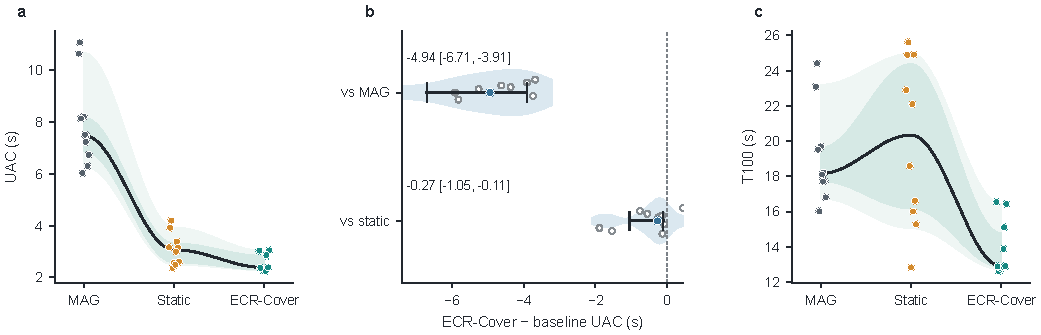
\includegraphics[width=\textwidth]{figure3_nominal.pdf}
\caption{Nominal hardware results, with ten block-level runs per method. (a,c) Run-level UAC and T100 observations; the dark and light envelopes denote the interquartile and 10th--90th percentile ranges, respectively, and the solid curve denotes the median. (b) Block-level paired UAC differences with descriptive density silhouettes and the frozen median 95\% bootstrap confidence intervals for ECR-Cover relative to MAG and calibrated static planning. The silhouettes are distributional summaries, not confidence regions.}\label{fig:nominal}
\end{figure*}

\subsection{Temporary Interruption and Repair Ablation}

In the interrupted system-level comparison, median UAC was 3.907~s for ECR-Cover and 5.617~s for calibrated static planning. The paired difference was $-1.134$~s, but its 95\% CI, $[-3.581,1.134]$~s, crossed zero. Median T100 values were 37.866 and 37.302~s. Because the two conditions used different initial routes and differed in online repair, this comparison cannot assign the observed difference specifically to repair. It instead characterizes complete methods under the same pause rule.

The repair switch ablation isolates the mechanism. With the same initial plan and interruption rule, repair-on UAC had a median of 3.549~s and repair-off UAC a median of 5.510~s. The paired median difference was $-1.979$~s with a 95\% CI of $[-2.496,-1.821]$~s. Nine blocks improved and one block was adverse; all ten appear in Figure~\ref{fig:repair}a. The preregistered one-sided exact sign test gave $p=0.010742$. Thus the effect is supported by the direction and interval of run-level paired observations, not by treating cells or control samples as independent replicates.

Repair-on median T95 was 20.206~s, compared with 38.001~s when repair was disabled. Median T100 values were 37.965 and 38.007~s. The paired T100 ratio had a median of 0.998 and a 95\% CI of $[0.954,1.0001]$. Its upper confidence bound was below the preregistered 1.05 noninferiority margin (Figure~\ref{fig:repair}b). The repair-on UAC improvement therefore occurred without evidence of a completion-time penalty beyond that margin.

Each repair-on run committed one effective repair and confirmed at least one reassigned cell before the paused camera recovered. No repair-off run contained such an event. The result supplies the physical witness required to connect Proposition~\ref{prop:repair}'s predicted commit rule to execution: the transferred task was not merely present in a modified queue; it produced a fresh-frame, measured-pose coverage record while the original device was still unavailable.

\begin{figure*}[t]
\centering
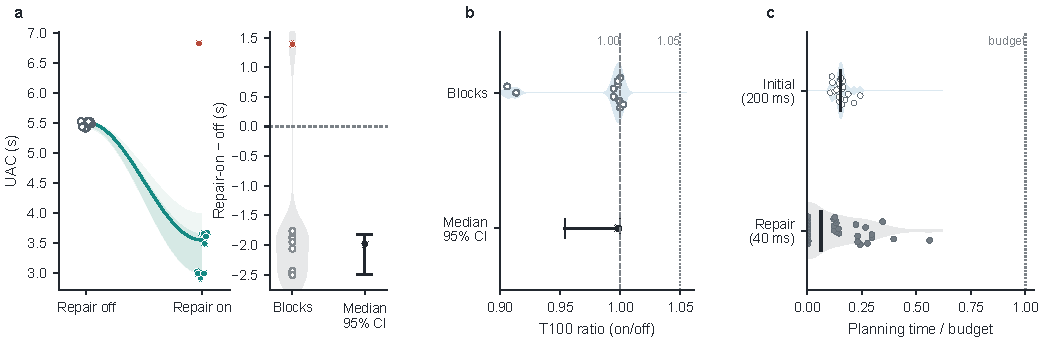
\includegraphics[width=\textwidth]{figure4_repair.pdf}
\caption{Repair ablation and computation budget. (a) Repair-off/on UAC observations with median trajectory and descriptive quantile envelopes; the adjacent axis retains all ten paired differences, including the single adverse block, and the frozen median 95\% bootstrap interval. (b) Block-level T100 ratios with a descriptive density silhouette and the frozen median interval; reference lines mark equality at 1.00 and the 5\% noninferiority boundary at 1.05. (c) All observed planning times normalized by their respective budgets, with descriptive density silhouettes and median ticks. Shaded envelopes and silhouettes are not confidence regions.}\label{fig:repair}
\end{figure*}

\subsection{Execution-Evidence Audit and Computation Budget}

The 70 runs generated 461 coverage-confirmation events. Median absolute azimuth and elevation differences between planned and confirming poses were both $0.5^\circ$; their 95th percentiles were both $0.9^\circ$, and no confirming event exceeded the $1^\circ$ completion gate. Within the frozen projection model, every one of the 461 planning-core cell sets was contained in the field of view projected from the corresponding measured pose, and every logged coverage cell belonged to that measured-pose projection. The planning core and measured-pose footprint contained median counts of 63 and 180 cells, respectively. These checks support consistency between software evidence and the frozen geometry; they do not add an external world-coordinate calibration.

All frames referenced by coverage events passed the logged usability and resolution checks and could be joined to the pose sample, frame identifier, task identifier, and COMPLETE event. One raw unusable-frame status occurred in the repair-ablation archive, but it was not referenced by a coverage event. The ledger therefore reconstructs all reported first-coverage times from qualifying execution events rather than scheduled timestamps.

Across the 20 repair-ablation runs, initial planning time ranged from 21.52 to 48.79~ms, with a median of 30.75~ms, below the 200~ms budget. The 40 pause/recovery planning events ranged from 0.10 to 22.48~ms, with a median of 2.56~ms, below the 40~ms event budget. Figure~\ref{fig:repair}c shows the observations relative to their respective budgets. These measurements establish budget compliance in the frozen Windows/Python platform; they are not a hard real-time schedulability result.


\section{Discussion}\label{sec:discussion}

\subsection{Closing the Planning--Execution Gap}

The experiments support the central distinction behind ECR-Cover: planned pointing and effective physical observation are different events. The nominal results show that a planner built around end-to-end confirmation time can change the complete first-coverage trajectory, not only the geometric route. MAG remained an executable reference and supplied a deterministic planning bound, yet ECR-Cover's paired hardware UAC was lower in every nominal block and its T100 tail was shorter. The smaller but resolved UAC difference from calibrated static planning indicates that part of the improvement comes from using a measured execution model and part from the subsequent baseline-preserving route search. These conclusions are empirical; Proposition~\ref{prop:initial} alone guarantees only that the planner did not accept a worse robust model objective.

The repair ablation provides a more direct causal comparison because the initial plan, interruption rule, and confirmation pipeline were held fixed. Repair reduced UAC in nine of ten blocks while the T100-ratio interval remained inside the noninferiority boundary. The adverse block is important: baseline-preserving model acceptance does not eliminate run-to-run execution variation. Its inclusion shows why physical superiority must be evaluated from independent paired runs rather than inferred from the planning rule. At the same time, the pre-recovery witnesses demonstrate that the observed aggregate effect corresponds to actual reassignment. Every repair-on run produced at least one confirmed cell from a migrated task before the paused device returned.

The execution ledger changes what can be claimed from a coverage experiment. A nominal arrival schedule would have supplied a smooth coverage curve but no proof that its steps corresponded to images. Here, each step can be joined to a successful command path, a stability interval, a fresh usable frame, a synchronized measured pose, and a cell projection. This evidence is especially relevant for networked cameras because the control and video paths do not share a single completion signal. ACK, arrival, and frame freshness must be represented separately. The ledger does not make the camera model exact; it makes the relationship between the model and recorded events explicit.

The UAC objective also reveals behavior that makespan alone would hide. ECR-Cover and calibrated static planning had similar nominal T95, yet their UAC and T100 differed. In repair ablation, the main benefit appeared in UAC and T95 while T100 stayed nearly unchanged. This pattern is consistent with moving useful observations earlier without necessarily changing the final interrupted task. The higher load CV shows the accompanying allocation choice: first-observation latency may favor a camera that can acquire a large set early, even when equal task counts would appear more balanced. Because that tradeoff was encoded before the experiment, it is an outcome of the objective rather than a post hoc explanation.

\subsection{Relationship Among Formal and Empirical Evidence}

The results form three evidence layers. The first layer is planning structure. Retaining MAG and the original residual queues makes nonreplacement observable: a time-limited search can always return a complete, already evaluated plan. Equations~\eqref{eq:initial-accept} and \eqref{eq:repair-accept} then give the respective model-relative inequalities. This layer is deterministic once the admissible map and time bounds are fixed.

The second layer is implementation consistency. The state machine and ledger ensure that a coverage write has the fields required by Proposition~\ref{prop:evidence}. The 461-event audit verifies that the frozen implementation followed this rule in all formal runs. Conditional completeness is likewise matched by the observed deployment: the admissible candidates jointly covered all 384 cells, every logical pause ended, and every run reached 384/384 confirmed cells. This observation verifies the premises in the tested setting, not for arbitrary future hardware faults.

The third layer is run-level physical statistics. Paired nominal blocks test whether model-relative planning improvement survives device dynamics and network timing. Repair-on/off blocks test whether the event mechanism improves the realized trajectory. Confidence intervals and sign tests belong to this layer. They neither prove the deterministic propositions nor become consequences of them. Conversely, a significant paired result cannot replace the baseline-preservation proof, because it does not prevent an individual future planning search from accepting a worse modeled plan. The value of ECR-Cover lies in combining the layers without collapsing their meanings.

The four-corner planning core illustrates the need for this separation. Offline sensitivity shows that a $1^\circ$ contraction materially changes candidate set sizes and task counts. It is therefore not a negligible numerical detail. Nevertheless, it remains a particular feasible-map construction. The initial and repair properties would apply to a different common map, while the external accuracy of either map would require independent geometric calibration. Presenting the core as a control-coordinate planning margin, rather than as a physical confidence region, preserves what the data actually support.

\subsection{Limitations}

Eight limitations delimit the present evidence. First, coverage is evaluated in one frozen local geometry. Station positions, mounting rotations, and individual camera intrinsics were not validated against external target ground truth, so model-consistent projection is not the same as absolute world-coordinate accuracy. Second, the $1^\circ$ four-corner intersection is linked to the pose-completion gate and measured telemetry errors; it does not jointly quantify every source of field-of-view uncertainty.

Third, no target trajectory or detection ground truth was available. UAC therefore measures first spatial observation opportunities. It can be interpreted as truncated expected detection delay only under the stationary, uniformly located, certain-detection assumptions stated in Section~\ref{sec:problem}. Fourth, the end-to-end timing margins depend on the relevance of the stratified calibration runs. The 89.6\% independent empirical coverage is consistent with the selected level but does not guarantee performance under nonstationary congestion, altered streaming parameters, or a different device population.

Fifth, the deployment contains four cameras at one site. It does not establish behavior for larger teams, heterogeneous cameras, or geometries with substantially different overlap. Sixth, the formal missions are minute-scale. Long-term thermal drift, encoder bias, camera restart behavior, and multi-day network variability were not tested. Seventh, unavailability was introduced as a controlled logical pause. The protocol tests residual-task reassignment and recovery timing, but it does not cover mechanical damage, corrupted telemetry, partial video degradation, or an unreachable device that never returns.

Eighth, planning was centralized on a soft real-time Windows/Python stack. The measured 200 and 40~ms budgets were met in the frozen experiment, but the data do not establish hard real-time deadlines, distributed consensus behavior, or communication contention in a larger network. These limitations identify the evidence needed for broader deployment claims: external geometric calibration, target-level validation, persistent-fault protocols, larger networks, and longer-duration trials. They are not addressed by expanding the interpretation of the current 70 runs.


\section{Conclusion}\label{sec:conclusion}

ECR-Cover addresses a specific weakness in cooperative sensing with networked directional cameras: a scheduled pointing direction is not evidence that an observation occurred. The method links a first-coverage objective to end-to-end execution-time bounds, retains executable baselines during initial search and event repair, and updates realized coverage only from a stable measured pose associated with a fresh usable frame.

On four ZR10 cameras, the frozen hardware study connected each formal property to a separate observable consequence. Initial planning preserved its MAG model baseline and produced lower paired nominal UAC and T100 in hardware. The execution ledger accounted for all 461 coverage events. Repair-on/off pairs showed lower first-coverage latency, T100 noninferiority, and a confirmed reassigned observation before recovery in every repair-on run. The results support an execution-confirmed coverage loop for this deployment; they do not establish target-detection probability or performance beyond the tested geometry, duration, and network scale.

The main design lesson is that planning, physical execution, and observation evidence should remain distinct until a validated event connects them. That separation allows route improvement to be bounded by an executable alternative and allows coverage performance to be reconstructed from what the sensors actually observed.



\bmsubsection*{Acknowledgments}
[ACKNOWLEDGMENTS TO BE COMPLETED AFTER DE-ANONYMIZATION.]

\bmsubsection*{Author Contributions}
[AUTHOR CONTRIBUTIONS TO BE COMPLETED AFTER DE-ANONYMIZATION.]

\bmsubsection*{Funding}
[FUNDING SOURCES AND GRANT NUMBERS TO BE COMPLETED.]

\bmsubsection*{Conflict of Interest}
[CONFLICT-OF-INTEREST STATEMENT TO BE CONFIRMED BY ALL AUTHORS.]

\bmsubsection*{Data Availability Statement}
[REPOSITORY URL, ACCESS CONDITIONS, AND RELEASE TIMING TO BE COMPLETED. The intended public release comprises the coverage-planning code, frozen configurations, run-level data, analysis scripts, and reproducible figure scripts, subject to the authors' final repository audit.]

\bmsubsection*{Generative AI Use Disclosure}
[DISCLOSURE TO BE CONFIRMED BY THE AUTHORS. A compliant statement should identify any generative-AI tools used for language editing or manuscript preparation, describe human verification of all technical content and citations, and state that the authors retain full responsibility for the manuscript.]

\bibliography{references}

\end{document}

